%!TeX root=../document.tex

\chapter{Solving the Equations of Motion}

\section{Static Solution}

\textcolor{red}{Static solution in context of bow: Bracing and equilibrium path, necessity for load control and displacement control}

A System with the equation of motion

\begin{align}
\boldsymbol{M}\,\ddot{\boldsymbol{u}} + \boldsymbol{q}(\boldsymbol{u},\,\dot{\boldsymbol{u}}) = \boldsymbol{p}
\end{align}

is in static equilibrium if~$\dot{\boldsymbol{u}},\,\ddot{\boldsymbol{u}} = \boldsymbol{0}$, leading to the static equilibrium condition

\begin{align}
\boldsymbol{q}(\boldsymbol{u},\,\boldsymbol{0}) = \boldsymbol{p}\label{eq:statics:equilibrium}
\end{align}

for the displacements $\boldsymbol{u}$ and the external loads $\boldsymbol{p}$.
This is a nonlinear system of equations and can be interpreted as the internal elastic forces~$\boldsymbol{q}$ being in balance with the external loads.

\subsection{The Basic Newton-Raphson Method}

Most frequently, when solving static problems, the external loads are given and the task is to calculate the corresponding equilibrium displacements.
Equation~(\ref{eq:statics:equilibrium}) is then a nonlinear system of equations in $\boldsymbol{u}$. Solving it can only be done numerically except for very simple examples.

An often used method for this kind of problem is the Newton-Raphson method. The basic idea behind it is to linearise the equilibrium equation~(\ref{eq:statics:equilibrium}) around a known displacement vector~$\boldsymbol{u}_i$ and solve the resulting linear equation to obtain an improved approximation~$\boldsymbol{u}_{i+1}$. Starting with an initial value~$\boldsymbol{u}_0$ the procedure is repeated until the solution is accurate enough by some convergence criterion.

Linearising of (\ref{eq:statics:equilibrium}) yields

\begin{align}
\boldsymbol{q}(\boldsymbol{u}_i) +
\underbrace{
\left(\frac{\partial \boldsymbol{q}}{\partial \boldsymbol{u}}\bigg \vert_{\boldsymbol{u}_i}\right)
}_{\boldsymbol{K}(\boldsymbol{u}_i)}
\underbrace{
(\boldsymbol{u}_{i+1} - \boldsymbol{u}_i)
}_{\Delta\boldsymbol{u}_i} &= \boldsymbol{p}
\end{align}

Solving for $\Delta\boldsymbol{u}_i$ leads to the iterative procedure

\begin{align}
\Delta\boldsymbol{u}_i &= \boldsymbol{K}^{-1}(\boldsymbol{u}_i)\left(\boldsymbol{p} - \boldsymbol{q}(\boldsymbol{u}_i)\right),\\
\boldsymbol{u}_{i+1} &= \boldsymbol{u}_i + \Delta\boldsymbol{u}_i.\label{eq:statics:newton_iteration}
\end{align}

In the implementation the tangent stiffness matrix is not actually inverted, because that's expensive and potentially inaccurate. Instead,~$\Delta\boldsymbol{u}_i$ is obtained by solving the equivalent linear system of equations using a decomposition of the stiffness matrix.
Since it is symmetrix, an algorithm that exploits this can be selected.
(The tangent stiffness matrix isn't necessarily positive definite though, unlike the stiffness matrices of some linear mechanical systems.)

In order to stop the iteration when an acceptable level of accuracy is reached, we need a stopping or convergence criterion.
Convergence criteria are commonly formulated in terms of either the displacement step $\Delta\boldsymbol{u}$, the residuum forces $\boldsymbol{p} - \boldsymbol{q}$ or a combination of both.
For our purposes we will use the displacement-based criterion

\begin{equation}
| \Delta\boldsymbol{u}_{i} | \ < \ \varepsilon_{\mathrm{rel}} \cdot | \boldsymbol{u}_{i} | \ + \ \varepsilon_{\mathrm{abs}}\label{eq:convergence_basic}
\end{equation}

where $| \cdot |$ denotes the coefficient-wise absolute value and~$\varepsilon_{\mathrm{rel}}$ and~$\varepsilon_{\mathrm{abs}}$ are relative and absolute error tolerances.
Doing a coefficient-wise, relative comparison of the displacement step with the current displacement vector as a reference avoids scaling problems, since the coefficients of~$\boldsymbol{u}$ can have different units and magnitude.
The absolute error tolerance~$\varepsilon_{\mathrm{abs}}$ is needed when one or more reference displacements are zero.
It is typically chosen much smaller than the relative error tolerance~$\varepsilon_{\mathrm{rel}}$.

The basic Newton-Raphson method can be improved and extended in many ways, for example by combining it with a line search or by avoiding the calculation of the tangent stiffness matrix at every iteration (simplified Newton-Raphson method, BFGS method \textcolor{red}{[Source]}).

\subsection{Constrained Newton-Raphson method}

In the previous section the Newton-Raphson method was applied to the problem of calculating the equilibrium displacements of a system when all applied forces are known. This method is used in VirtualBow for finding the braced equilibrium state of the bow (see section \textcolor{red}{[Reference]}). However, when calculating the draw curve we don't actually know the draw forces, just the displacement of the string center. \textcolor{red}{Also: Load decrease.}

A solution to this is displacement control, where we prescribe a value for one of the displacement components and instead treat the corresponding external forces as a variable that is determined during solution.

The following derivation has been adapted from \cite{fem_script_uni_bochum}. Displacement control is a special case of a wider class of methods where the equilibrium equations are modified as
%
\begin{align}
\boldsymbol{q}(\boldsymbol{u}) - \lambda\,\boldsymbol{p} &= 0,\label{eq:equilibrium_dc}\\
c(\boldsymbol{u},\,\lambda) &= 0.\label{eq:constraint_dc}
\end{align}
%
Here the external forces are scaled by the unknown load factor $\lambda$. To compensate for this additional unknown, a scalar constraint~$c(\boldsymbol{u},\,\lambda) = 0$ on the displacements and the load parameter is introduced. Depending on the choice of constraint the method can be turned into load control, displacement control or other more sophisticated schemes like the arc-length method. We will carry out the derivation for the general case and specify the constraints later. This is also how these methods are implemented in VirtualBow: A general implementation for arbitrary constraints that is then specialized into load controlled and displacement controlled methods by providing the necessary constraints.

The system of nonlinear equations (\ref{eq:equilibrium_dc}), (\ref{eq:constraint_dc}) has to be solved for the displacements~$\boldsymbol{u}$ and the load parameter~$\lambda$. Like before, the Newton-Raphson method is used: The equations are linearised around a given approximation~$\{\boldsymbol{u}_i,\,\lambda_i\}$ and solved to obtain an improved approximiation~$\{\boldsymbol{u}_{i+1},\,\lambda_{i+1}\}$. This is repeated iteratively until displacements and load parameter satisfy the equilibrium equations~(\ref{eq:equilibrium_dc}) as well as the constraint equation~(\ref{eq:constraint_dc}) reasonably well as determined by some convergence criterion.

Carrying out the linearisation leads to the two equations
%
\begin{align}
\boldsymbol{q}(\boldsymbol{u}) - \lambda\,\boldsymbol{p}\:&\approx\:\boldsymbol{q}(\boldsymbol{u_{i}}) - \lambda_i\,\boldsymbol{p} + 
\underbrace{
\frac{\partial \boldsymbol{q}}{\partial \boldsymbol{u}}(\boldsymbol{u_{i}})
}_{\boldsymbol{K_{i}}}
\underbrace{
(\boldsymbol{u_{i+1}} - \boldsymbol{u_{i}})
}_{\Delta\boldsymbol{u_{i}}}
- \boldsymbol{p}
\underbrace{
\,(\lambda_{i+1} - \lambda_{i})
}_{\Delta \lambda_{i}}
\notag\\
&\approx\ \boldsymbol{q}(\boldsymbol{u_{i}}) - \lambda_i\,\boldsymbol{p} + \boldsymbol{K_{i}}\,\Delta\boldsymbol{u_{i}} - \boldsymbol{p}\,\Delta \lambda_{i}\label{eq:equilibrium_dc_lin}\\
\notag\\
c(\boldsymbol{u},\,\lambda) \ &\approx\ c(\boldsymbol{u_{i}},\,\lambda_{i}) + \frac{\partial c}{\partial \boldsymbol{u}}(\boldsymbol{u_{i}},\,\lambda_{i})(\boldsymbol{u_{i+1}} - \boldsymbol{u_{i}}) + \frac{\partial c}{\partial \lambda}(\boldsymbol{u_{i}},\,\lambda_{i})(\lambda_{i+1} - \lambda_{i})\notag\\
&\approx\ c(\boldsymbol{u_{i}},\,\lambda_{i}) + \frac{\partial c}{\partial \boldsymbol{u}}(\boldsymbol{u_{i}},\,\lambda_{i})\,\Delta\boldsymbol{u_{i}} + \frac{\partial c}{\partial \lambda}(\boldsymbol{u_{i}},\,\lambda_{i})\,\Delta \lambda_{i}\label{eq:constraints_dc_lin}
\end{align}

Equations~(\ref{eq:equilibrium_dc_lin}) and~(\ref{eq:constraints_dc_lin}) can written as the single linear system of equations
%
\begin{align}
\begin{bmatrix}
\boldsymbol{K_{i}} & -\boldsymbol{p}\\
\frac{\partial c}{\partial \boldsymbol{u}}(\boldsymbol{u_{i}},\,\lambda_{i}) & \frac{\partial c}{\partial \lambda}(\boldsymbol{u_{i}},\,\lambda_{i})
\end{bmatrix}
\begin{bmatrix}
\Delta\boldsymbol{u_{i}}\\
\Delta \lambda_{i}
\end{bmatrix}
=
\begin{bmatrix}
\lambda_i\,\boldsymbol{p} - \boldsymbol{q}(\boldsymbol{u_{i}})\\
-\boldsymbol{c}(\boldsymbol{u_{i}},\,f_{i})
\end{bmatrix}.\label{eq:total_dc_lin}
\end{align}
%
Solving this for the increments in displacement and load factor $\{\Delta\boldsymbol{u_{i}},\,\Delta \lambda_{i}\}$ allows us to calculate the next values as
%
\begin{align}
\boldsymbol{u_{i+1}} = \boldsymbol{u_{i}} + \Delta\boldsymbol{u_{i}}\\
\lambda_{i+1} = \lambda_{i} + \Delta \lambda_{i}.
\end{align}
%
However, directly solving~(\ref{eq:total_dc_lin}) is not  numerically efficient because the augmented stiffness matrix is no longer symmetric. A much better way to solve this is block elimination. We use the first row of~(\ref{eq:total_dc_lin}) to express~$\Delta\boldsymbol{u_{i}}$ as
%
\begin{align}
\Delta\boldsymbol{u_{i}} &= \boldsymbol{\alpha} + \boldsymbol{\beta}\,\Delta \lambda_{i}.\label{eq:auxiliary_disp_dc}
\end{align}
%
With the auxiliary vectors
%
\begin{align}
\boldsymbol{\alpha} &= \boldsymbol{K_{i}^{-1}}(\lambda_i\,\boldsymbol{p} - \boldsymbol{q}(\boldsymbol{u_{i}}))\label{eq:auxiliary_1}\\
\boldsymbol{\beta} &= \boldsymbol{K_{i}^{-1}}\,\boldsymbol{p}\label{eq:auxiliary_2}
\end{align}
%
These can be computed efficiently by exploiting the symmetry of the stiffness matrix $\boldsymbol{K_{i}}$.
%
To calculate $\Delta \lambda_i$, we substitute~(\ref{eq:auxiliary_disp_dc}) into the second row of~(\ref{eq:total_dc_lin}) which gives us
%
\begin{align}
&\frac{\partial c}{\partial \boldsymbol{u}}(\boldsymbol{u_{i}},\,\lambda_{i})\Delta\boldsymbol{u_{i}} + \frac{\partial c}{\partial \lambda}(\boldsymbol{u_{i}},\,\lambda_{i})\,\Delta \lambda_{i} = -c(\boldsymbol{u_{i}},\,\lambda_{i})\notag\\
&\frac{\partial c}{\partial \boldsymbol{u}}(\boldsymbol{u_{i}},\,\lambda_{i})(\boldsymbol{\alpha} + \boldsymbol{\beta}\,\Delta \lambda_{i}) + \frac{\partial c}{\partial \lambda}(\boldsymbol{u_{i}},\,\lambda_{i})\,\Delta \lambda_{i} = -c(\boldsymbol{u_{i}},\,\lambda_{i})\notag\\
&\ \ \vdots\notag\\
&\Delta \lambda_{i} = -\frac{c(\boldsymbol{u_{i}},\,\lambda_{i}) + \frac{\partial c}{\partial \boldsymbol{u}}(\boldsymbol{u_{i}},\,\lambda_{i})^\intercal\,\boldsymbol{\alpha}}{\frac{\partial c}{\partial \lambda}(\boldsymbol{u_{i}},\,\lambda_{i}) + \frac{\partial c}{\partial \boldsymbol{u}}(\boldsymbol{u_{i}},\,\lambda_{i})^\intercal\,\boldsymbol{\beta}}.\label{eq:res_load_factor}
\end{align}

To summarize: First, calculate $\boldsymbol{\alpha}$ and~$\boldsymbol{\beta}$ by solving~(\ref{eq:auxiliary_1}) and~(\ref{eq:auxiliary_2}). Then calculate the increment of the load parameter by using~(\ref{eq:res_load_factor}). The increment in displacements is then obtained by equation~(\ref{eq:auxiliary_disp_dc}).

From equation (\ref{eq:res_load_factor}) we can see that the load factor increment $\Delta \lambda_{i}$ is invalid if $\frac{\partial c}{\partial \lambda} + \frac{\partial c}{\partial \boldsymbol{u}}^\intercal\,\boldsymbol{\beta} = 0$, i.e. the denominator of the expression vanishes.
This needs to be checked by the implementation and usually points to an ill-posed problem with regards to the imposed constraint function.


Applying the convergence criterion (\ref{eq:convergence_basic}) from the base method to (\ref{eq:total_dc_lin}) is equivalent to the two criteria
%
\begin{align}
| \Delta\boldsymbol{u}_{i} | \ &< \ \varepsilon_{\mathrm{rel}} \cdot | \boldsymbol{u}_{i} | \ + \ \varepsilon_{\mathrm{abs}}, \\
| \Delta \lambda_{i} | \ &< \ \varepsilon_{\mathrm{rel}} \cdot | \lambda_{i} | \ + \ \varepsilon_{\mathrm{abs}},
\end{align}

both of which must be satisfied in order for the iteration to be stopped.

\subsection{Constraints for load- and displacement control}

Finally, the constraint function has to be chosen.
To get a displacement controlled method as initially stated we choose the constraint function as
%
\begin{align}
\boldsymbol{c}(\boldsymbol{u},\,\lambda) = u^{(k)} - \overline{u}
\end{align}
%
where~$u^k$ is the $k$-th component of the displacement vector that we want to control and $\overline{u}$ is the prescribed value for it. The partial derivatives are
%
\begin{align*}
\frac{\partial c}{\partial \boldsymbol{u}} &= \boldsymbol{e}_k,\quad
\frac{\partial c}{\partial \lambda} = 0,
\end{align*}
%
with $\boldsymbol{e}_k$ being the $k$-th unit vector. If a load controlled method is needed instead, the constraint becomes
%
\begin{align}
\boldsymbol{c}(\boldsymbol{u},\,\lambda) = \lambda - \overline{\lambda},
\end{align}
%
with the desired load factor $\overline{\lambda}$. Partial derivatives:
%
\begin{align*}
\frac{\partial c}{\partial \boldsymbol{u}} &= \boldsymbol{0},\quad
\frac{\partial c}{\partial \lambda} = 1,
\end{align*}

\subsection{Line search}

There is one last extension to the Newton-Raphson method that is needed for our purposes and that is line search. 

\textcolor{red}{Todo: Explain line search and why it helps with contact handling}

\subsection{Equilibrium paths and step size control}

With the displacement controlled Newton-Raphson method we can solve for static equilibrium at any given displacement.
We often want to do this repeatedly for a whole range of target displacements.
The static simulation of the bow, for example, produces a series of equilibrium states from brace height to full draw from which things like the force-draw curve can be extracted.
Even if the intermediate states were of no interest, sometimes the target displacement may be too far from the initial displacement such that the Newton-Raphson iterations only converge if multiple smaller displacement steps are being made.

The easiest way to do this is to use a fixed number of equal displacement steps.
This works fine as long as there is good converge at each step.
However, during some part of this equilibrium path the step size might be too large so that there is either no convergence or many iterations are needed at each step.
In this case we would like to decrease the step size temporarily.
Conversely, if convergence gets better we would like to increase the displacement step again for efficiency.
This adaption is called step size control.

The method used in VirtualBow first calculates a lower and upper bound on the displacement step as
%
\begin{align}
\Delta u_\mathrm{min} &= \frac{u_\mathrm{target} - u_\mathrm{start}}{n_\mathrm{max}}, \\
\Delta u_\mathrm{max} &= \frac{u_\mathrm{target} - u_\mathrm{start}}{n_\mathrm{min}}.
\end{align}

Here,~$n_\mathrm{min}$ and~$n_\mathrm{max}$ are parameters that determine the minimum number of steps in the output as well as the maximum number of steps before the procedure is aborted.
Another required parameter is the desired number of iterations $\mathrm{iter\_target}$ at each displacement step.

We start the step size control with the maximum step of~$\Delta u = \Delta u_\mathrm{max}$.
After performing the Newton-Raphson iterations we adjust the step size depending on whether the iteration was successful or not.

\textbf{Success:} If the iterations converged, the step size is adjusted based on the number of iterations $\mathrm{iter\_actual}$ that were needed and the desired number of iterations $\mathrm{iter\_target}$:
%
$$
\Delta u := \mathrm{clamp} \left\lbrace \Delta u \sqrt{\frac{\mathrm{iter\_target}}{\mathrm{iter\_actual}}},\,\Delta u_\mathrm{min},\,\Delta u_\mathrm{max} \right\rbrace
$$

In other words, the step size is decreased if more iterations than desired were needed and increased if fewer were needed.
Also the step size is never decreased below~$\Delta u_\mathrm{min}$ or increased above~$\Delta u_\mathrm{max}$.

\textbf{Failure:} In the case of iteration failure, the number of iterations can't be used to adjust the step size.
But we know that the step size has to be reduced in order to increase the chance for a successful iteration.
That's why it is multiplied with a reduction factor~$0 < r < 1$,
%
$$
\Delta u := r \cdot \Delta u.
$$

The simulation is aborted if there was a failure and the step size can not be decreased any further (because the lower bound~$\Delta u_\mathrm{min}$ was already reached).

\newpage
\subsection{Finding the Braced Equilibrium State}

The first part of the static simulation is also the most tricky one: Finding the first equilibrium state of the bow at the given brace height.
Especially older versions of VirtualBow would frequently struggle with this step and give users cryptic error messages from failed solution attempts.
The bracing method described in the following is the result of a lot of trial and error and seems to be the most robust so far, even though still not perfect.

One difficulty of bracing is that the braced state of the bow tends to be "far away" from the initial, unbraced state.
Newton-Raphson iterations however are much more efficient and robust when having a good initial guess, i.e. an initial state that is not very far from the desired equilibrium.
So ideally we would like to go from the unbraced to the braced state in a series of intermediate equilibrium states.
The other difficulty is that the length of the string is not known in advance, only the brace height that the bow should have when the string is applied.

The current bracing method tries to solve both of these problems by applying a string to the bow that is initially too long and iteratively shorten it until the desired brace height is reached.
By controlling/limiting how much the string is shortened in each step, the solution process is more likely to converge.

As shown in figure \ref{fig:bracing-method-1}, a string with initial length $l_{0}$ is applied to the unbraced configuration of the bow such that it passes through the desired brace height on the $y$ axis.
The initial length is chosen such that there is no tension yet in the string.

\begin{figure}[h]
\centering
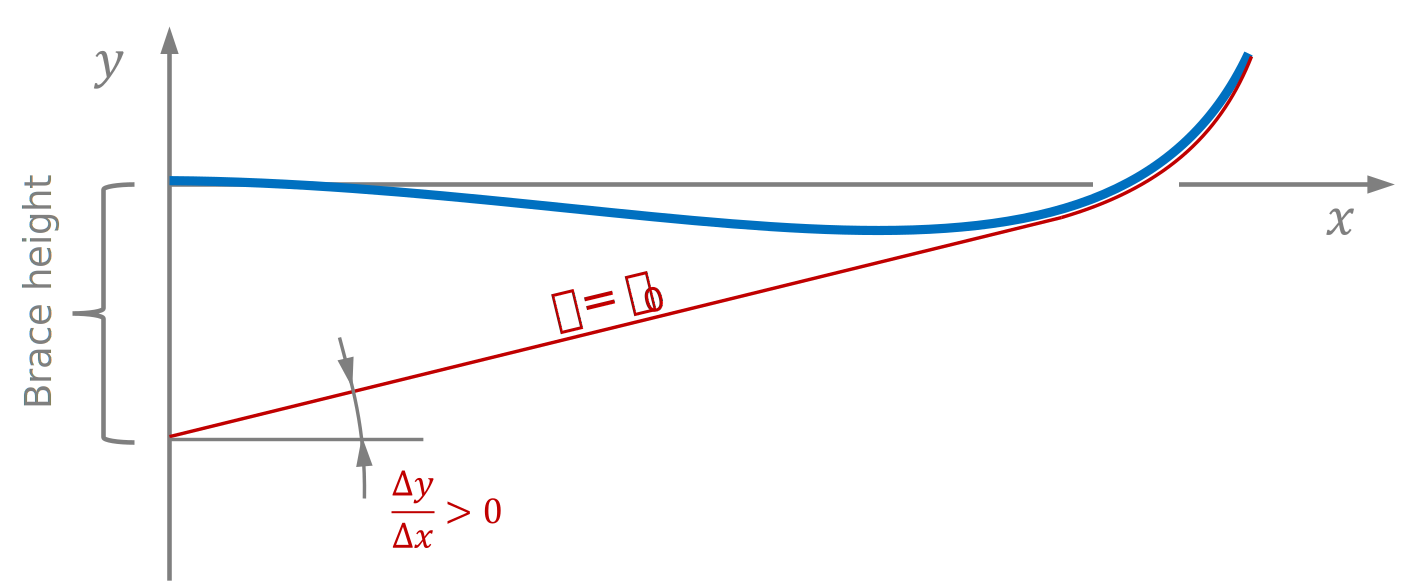
\includegraphics[width=0.7\textwidth]{figures/solution/bracing-method-1}
\caption{Unbraced state}
\label{fig:bracing-method-1}
\end{figure}

At the point where the string intersects the $y$ axis, it initially has a positive slope of $\Delta y / \Delta x$ as measured against the $x$ direction.
If this initial slope were negative, the bow model would have to be rejected as invalid because the specified brace height is too low for the given limb geometry.
The actual bracing process now consists of successively shortening the string and iterating for equilibrium until the slope reaches zero, while keeping the string center pinned at the desired brace height via displacement control.
This pinning of the string ensures a favorable angle (not too shallow) between string and limb.

\begin{figure}[h]
\centering
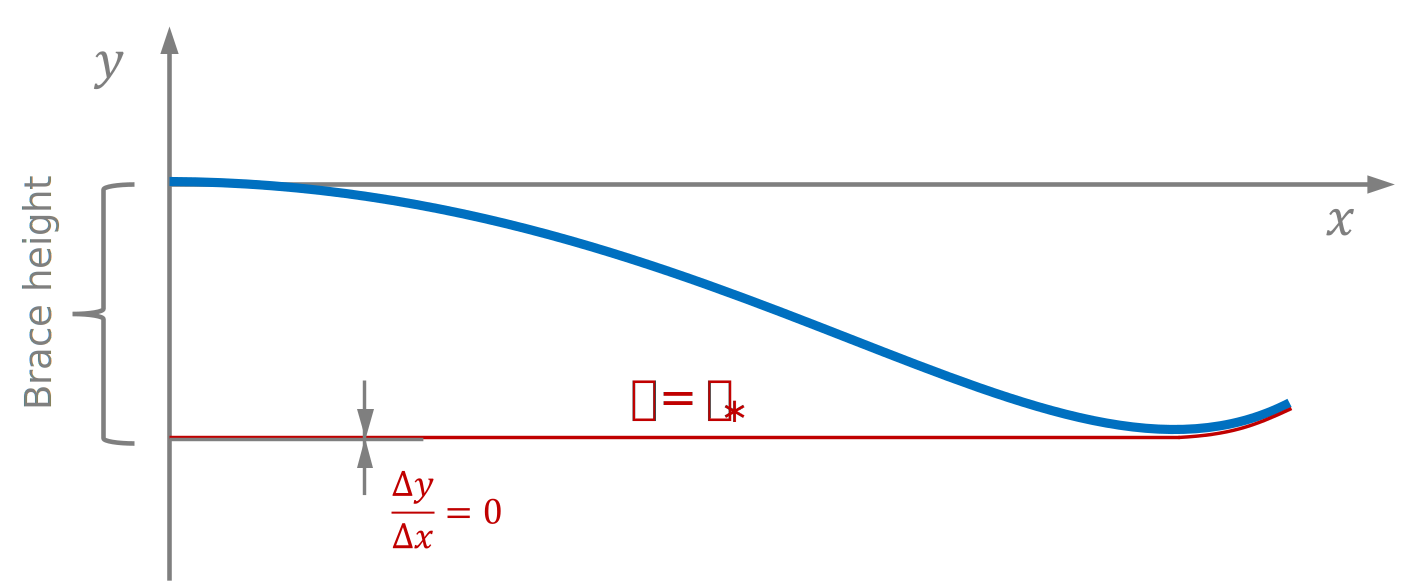
\includegraphics[width=0.7\textwidth]{figures/solution/bracing-method-2}
\caption{Braced state}
\label{fig:bracing-method-2}
\end{figure}

As the string becomes shorter, the slope decreases until it crosses into the negative.
The final string length $l_*$ is the length for which the slope is approximately zero.
This is shown in figure \ref{fig:bracing-method-2}.
So it all reduces to the problem of finding the root $\frac{\Delta y}{\Delta x}(l) = 0$ of the slope as a function of the string length.
This can be made dimensionless by introducing the length reduction factor $p = \frac{l}{l_{0}}$ and writing the slope as $\frac{\Delta y}{\Delta x}(p)$ instead.
Figure \ref{fig:bracing-plot} shows that relationship for a real example, where the final string length is found to be approximately~$0.96\,l_{0}$.

\begin{figure}[h]
\centering
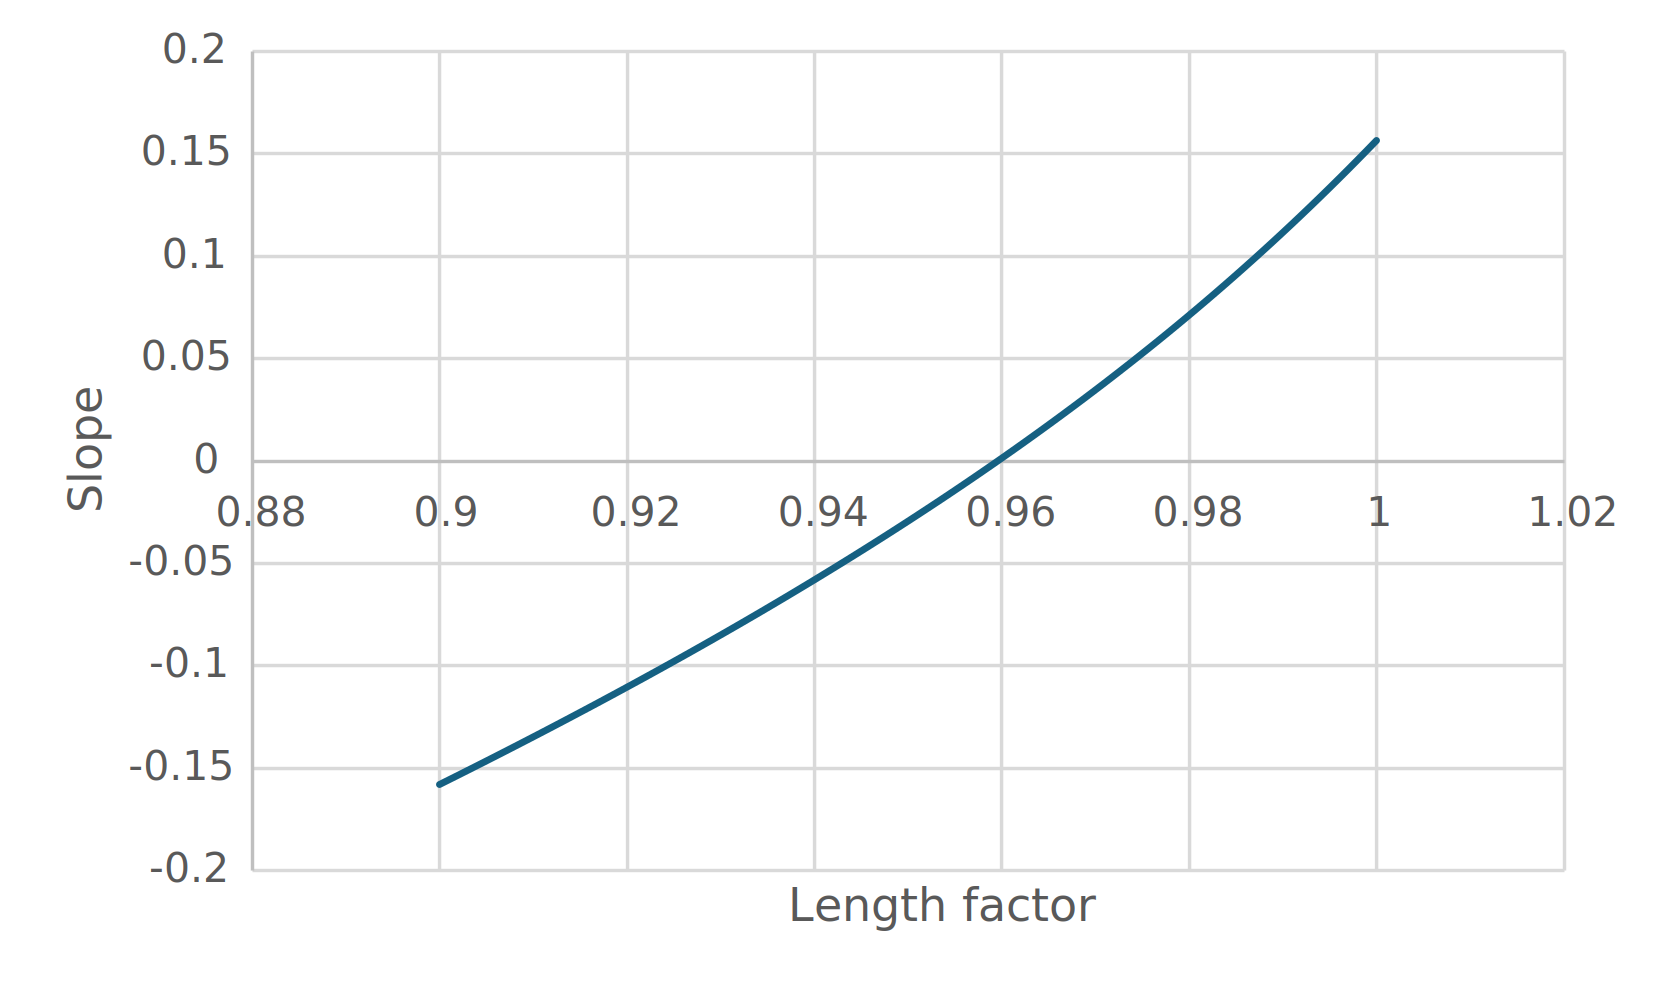
\includegraphics[width=0.6\textwidth]{figures/solution/bracing-plot}
\caption{Slope over string length for a real example}
\label{fig:bracing-plot}
\end{figure}

However, if we just use one of the many standard root finding algorithms for this, it might make big steps in string length and cause the underlying static Newton-Raphson iteration to fail.
Instead, the method starts at $p = 1$ and treats the problem like finding an equilibrium path with the path parameter $p$.
This parameter is controlled just as described in the previous section, taking into account maximum and minumum bounds on the step size and the performance of the static iterations.
A dedicated root finding algorithm is only used after the first negative slope is encountered in order to hone in on a precise final result.
Currently this is the regula falsi method, which is simple and effective when derivatives are not available and the interval in which the root lies is known.

\newpage
\section{Dynamic Solution}

The equations of motion of the system take the form of a second-order ordinary differential equation (ODE).
Together with the initial displacements~$\boldsymbol{u}_0$ and velocities~$\mathbf{v}_0$ at time $t_0$ they form the second-order initial value problem
%
\begin{align}
&\boldsymbol{M}\ddot{\boldsymbol{u}} + \boldsymbol{D}\dot{\boldsymbol{u}} + \boldsymbol{Q}(\boldsymbol{u}) = \boldsymbol{P}(t) \label{eq:dynamics:system_equation} \\
&\boldsymbol{u}(t_0) = \boldsymbol{u}_0 \\
&\dot{\boldsymbol{u}}(t_0) = \mathbf{v}_0
\end{align}

whose solution is the time progression~$\boldsymbol{u}(t),\,t > t_0$ of the displacements.
Since the ODE (\ref{eq:dynamics:system_equation}) is also nonlinear, there is no general analytical solution to this problem and we once again have to employ numerical methods.

Numerical solution of ODEs is an extensive topic and a large number of algorithms with different advantages and disadvantages is available.
Most general algorithms require equation~(\ref{eq:dynamics:system_equation}) to be transformed into an equivalent first order system of the form~$\dot{\boldsymbol{x}} = \boldsymbol{f}(\boldsymbol{x},\,t)$, with the state vector $\boldsymbol{x}(t)$ that combines the information of the displacements as well as the velocities.
The common choice of $\boldsymbol{x}(t) = (\boldsymbol{u}(t),\,\dot{\boldsymbol{u}}(t))^\intercal$ leads to the first order ODE

\begin{equation}
\frac{d}{dt}
\underbrace{
\begin{bmatrix}
\boldsymbol{u}(t) \\
\dot{\boldsymbol{u}}(t)
\end{bmatrix}
}_{\boldsymbol{x}(t)}
=
\underbrace{
\begin{bmatrix}
\dot{\boldsymbol{u}}(t) \\
\boldsymbol{M}^{-1}\left(\boldsymbol{P}(t) - \boldsymbol{D}\dot{\boldsymbol{u}} - \boldsymbol{Q}(\boldsymbol{u})\right)
\end{bmatrix}
}_{\boldsymbol{f}(\boldsymbol{x},\,t)}.
\end{equation}

Early prototypes of VirtualBow followed this approach and solved the resulting first order problem with methods provided by the C++ library Odeint \cite{bib:ahnert2011}.
Especially the error controlled Runge-Kutta methods worked reasonably well.
In addition to those general methods, there are also numerous methods that have been developed with finite elements/structural dynamics in mind.
Those operate directly on the second order problem~(\ref{eq:dynamics:system_equation}) and are usually more effective for this type of problem.

All numerical methods for solving ODEs can be grouped into either explicit and implicit ones.
Explicit methods use the current state of the system at time~$t$ to calculate the next state at~$t + \Delta t$.
Implicit methods instead find the next state by solving an equation that involves the current as well as the next state.
In the context of finite element analysis, implicit methods require equilibrium iterations at every time step involving the system's tangent stiffness matrix, while explicit methods only require simple vector operations.
Implicit methods therefore have a higher computational cost per step, but can make up for it by requiring less steps overall, as their better stability allows them to use much larger step sizes than explicit methods.

Explicit methods are easier to implement and are a good choice for small time scales, like impact and wave propagation problems.
They are most effective when the computation of the time steps is fast, so they work well with constant, diagonal (lumped) mass matrices and simple elements with low-order shape functions.

Implicit methods in contrast are well suited for larger time scales, where explicit algorithms would need an excessive number of steps.
Examples are structural response problems or numerically stiff systems, i.e. systems whose eigenfrequencies range from very small to very large.

From version 0.1 to 0.9, VirtualBow used the explicit central difference method \cite{bib:bathe2006}, which is probably one of the most popular explicit methods in finite element analysis.
Later versions use the Generalized-$\alpha$ method instead, which is an implicit method and closely related to the also very popular Newmark-$\beta$ method.

\subsection{Newmark-$\boldsymbol{\beta}$ Method}

The continuous solution $\boldsymbol{u}(t)$ is approximated by the discrete values~$\boldsymbol{u}_i = \boldsymbol{u}(t_{i})$, with time steps of $\Delta t = t_{i+1} - t_{i}$ between the solution points.
The core of the Newmark method~\cite{bib:bathe2006} is a set of approximations that express the displacements $\boldsymbol{u}_{n+1}$ and velocities $\mathbf{v}_{n+1}$ at the next timestep in terms of the known state $\boldsymbol{u}_{n}$, $\mathbf{v}_{n}$, $\boldsymbol{a}_{n}$ at the previous timestep as well as the unknown acceleration~$\boldsymbol{a}_{n+1}$:
%
\begin{align}
&\boldsymbol{u}_{n+1} = \boldsymbol{u}_{n} + \Delta t\,\mathbf{v}_{n} + \Delta t^2 \left( \left(\nicefrac{1}{2} - \beta\right)\boldsymbol{a}_{n} + \beta\,\boldsymbol{a}_{n+1} \right) \label{eq:newmark_u} \\
&\mathbf{v}_{n+1} = \mathbf{v}_{n} + (1 - \gamma)\Delta t\,\boldsymbol{a}_{n} + \gamma\,\Delta t\,\boldsymbol{a}_{n+1} \label{eq:newmark_v}
\end{align}

The choice of the parameters $\beta$ and $\gamma$ determines how the acceleration is assumed to vary within the interval and leads to different variants of the scheme, e.g. $\beta = \frac{1}{4},\,\gamma = \frac{1}{2}$ for the average constant acceleration method or $\beta = \frac{1}{6},\,\gamma = \frac{1}{2}$ for the linear acceleration method.

With (\ref{eq:newmark_u}) and (\ref{eq:newmark_v}) there are two equations for the three unknowns $\boldsymbol{u}_{n+1}$, $\mathbf{v}_{n+1}$ and $\boldsymbol{a}_{n+1}$.
The third equation is obtained by applying the equation of motion (\ref{eq:dynamics:system_equation}) to the end of the interval,

\begin{equation}
\boldsymbol{M}\boldsymbol{a}_{n+1} + \boldsymbol{D}\mathbf{v}_{n+1} + \boldsymbol{Q}(\boldsymbol{u}_{n+1}) = \boldsymbol{P}(t_{n+1}). \label{eq:newmark_balance}
\end{equation}

This is what makes the method implicit, since an equation involving the current state as well as the yet unknown next state of the system has to be solved in each step.
Finding the accelerations $\boldsymbol{a}_{n+1}$ is equivalent to finding the root of the function

$$
\boldsymbol{F}(\boldsymbol{a}_{n+1}) = \boldsymbol{M}\boldsymbol{a}_{n+1} + \boldsymbol{D}\mathbf{v}_{n+1}(\boldsymbol{a}_{n+1}) + \boldsymbol{Q}(\boldsymbol{u}_{n+1}(\boldsymbol{a}_{n+1})) - \boldsymbol{P}(t_{n+1})
$$

which can be done with Newton-Raphson iterations very similar to the case of static equilibrium.
The jacobian matrix required for this can be calculated as

$$
\frac{\partial \boldsymbol{F}}{\partial \boldsymbol{a}_{n+1}} = \boldsymbol{M} + \gamma \Delta t \boldsymbol{D} + \beta \Delta t^2 \boldsymbol{K}(\boldsymbol{u}_{n+1}(\boldsymbol{a}_{n+1}))
$$

and includes the tangent stiffness matrix $\boldsymbol{K}$ of the system, together with other constant terms.


\subsection{Generalized-$\boldsymbol{\alpha}$ Method}

The Newmark method is the basis for various other methods that improve on some of its numerical properties.
One of those is the Generalized-$\alpha$ method~\cite{bib:chung1993}, which itself is a generalization of various other Newmark-derived schemes.
Its key improvement over the classical Newmark method is configurable numerical dissipation, i.e. damping of spurious oscillations in the high frequency range that are not properly resolved.

A good description and analysis of the method for the nonlinear case can be found in \cite{bib:erlicher2002}.

The Newmark approximations (\ref{eq:newmark_v}), (\ref{eq:newmark_u}) are used as before, but the balance equation~(\ref{eq:newmark_balance}) is modified to
%
\begin{equation}
\boldsymbol{M}\boldsymbol{a}_{n+1-\alpha_m} + \boldsymbol{D}\mathbf{v}_{n+1-\alpha_f} + \boldsymbol{Q}_{n+1-\alpha_f} = \boldsymbol{P}_{n+1-\alpha_f},
\end{equation}

so the equation of motion is not evaluated at the interval end~$t_{n+1}$ but at two points~$t_{n+1-\alpha_m}$ and~ $t_{n+1-\alpha_f}$ within the interval instead.
This can be configured with the additional parameters $\alpha_{m}$ and $\alpha_{f}$.
The intermediate displacements, velocities and accelerations are interpolated as
%
\begin{align}
\boldsymbol{u}_{i+1-\alpha_f} &= (1 - \alpha_f)\,\boldsymbol{u}_{i+1} + \alpha_f\boldsymbol{u}_{i} \\
\mathbf{v}_{i+1-\alpha_f} &= (1 - \alpha_f)\,\mathbf{v}_{i+1} + \alpha_f\mathbf{v}_{i} \\
\boldsymbol{a}_{i+1-\alpha_m} &= (1 - \alpha_m)\,\boldsymbol{a}_{i+1} + \alpha_m\boldsymbol{a}_{i}
\end{align}

For the evaluation of the forces there are several alternatives described in \cite{bib:erlicher2002}.
The most simple one, referred to by the authors as the \textit{generalized trapezoidal rule}, is
%
\begin{align}
\boldsymbol{Q}_{n+1-\alpha_f} =  (1 - \alpha_f)\,\boldsymbol{Q}_{i+1} + \alpha_f\boldsymbol{Q}_{i}, \\
\boldsymbol{P}_{n+1-\alpha_f} =  (1 - \alpha_f)\,\boldsymbol{P}_{i+1} + \alpha_f\boldsymbol{P}_{i}.
\end{align}

With this, the system of equations to solve in each iteration, including its jacobian matrix, becomes
%
\begin{align}
\boldsymbol{F}(\boldsymbol{a}_{n+1}) &= \boldsymbol{M}\boldsymbol{a}_{n+1-\alpha_m} + \boldsymbol{D}\mathbf{v}_{n+1-\alpha_f} + \boldsymbol{Q}_{n+1-\alpha_f} - \boldsymbol{P}_{n+1-\alpha_f}, \\
\frac{\partial \boldsymbol{F}}{\partial \boldsymbol{a}_{n+1}} &= (1 - \alpha_m)\boldsymbol{M} + (1 - \alpha_f)\left( \gamma \Delta t \boldsymbol{D} + \beta \Delta t^2 \boldsymbol{K}(\boldsymbol{u}_{n+1}(\boldsymbol{a}_{n+1})) \right).
\end{align}

The numerical damping of high-frequency modes is controlled with the spectral radius $\rho_{\infty} \in [0,\,1]$ at infinity.
A value of 1 corresponds to no numerical dissipation, while 0 corresponds to the so-called asymptotic annihilation of the high-frequency response.
The other constants are chosen as

\begin{equation}
\alpha_m = \frac{2\rho_{\infty} - 1}{\rho_{\infty} + 1},\quad \alpha_f = \frac{\rho_{\infty}}{\rho_{\infty} + 1},\quad \beta = \frac{1}{4}\left(1 - \alpha_m + \alpha_f\right)^2,\quad \gamma = \frac{1}{2} - \alpha_m + \alpha_f.
\end{equation}

These relations guarantee second order accuracy as well as unconditional stability in the linear case.

\newpage
\subsection{Adaptive time step}

In the previous sections the timestep $\Delta t$ was implicitly assumed to be constant.

\cite{bib:hulbert1995}

With $\Delta \boldsymbol{u} = \boldsymbol{u}_{i+1} - \boldsymbol{u}_{i}$

\begin{equation}
\omega^2 = \left\vert \frac{\Delta \boldsymbol{u}^\intercal \boldsymbol{K} \Delta \boldsymbol{u}}{\Delta \boldsymbol{u}^\intercal   \boldsymbol{M} \Delta \boldsymbol{u}} \right\vert, \quad T = \frac{2\pi}{\omega}
\end{equation}

\begin{equation}
\Delta t = \frac{T}{N}
\end{equation}

Other option:

\begin{equation}
\Delta t_{i+1} = \Delta t_{i} \cdot \sqrt{\frac{e_{\mathrm{target}}}{e_{\mathrm{actual}}}}
\end{equation}




\newpage
\subsection{Stopping Criterion and Progress Estimation}

The dynamic simulation is carried out until some stopping criterion is satisfied.
This criterion has to be chosen such that the simulated time interval contains all the information needed by the users while also keeping it as short as possible.
It has to include the separation of the arrow from the string plus some additional time, because some things like e.g. the maximum force on the string tend to happen only after the arrow left the bow.
A related requirement on the stopping criterion is that it must allow estimating the simulation progress, so that it can be shown to the user.

The simplest solution would be to simulate until a fixed time is reached.
This makes the progress estimation very easy, but it also has some drawbacks.
It would require users to specify the simulation time, which can only be found by trial and error and might have to be adjusted for different bows.

The current approach is to simulate the time interval~$[0,\,\alpha\,T]$ where~$T$ is the time for the arrow to reach brace height and~$\alpha$ is an arbitrary positive factor.
The default value is~$\alpha = 1.5$. The simulation progress at time~$\overline{t}$ can now be written as

\begin{equation}
\rm{progress} = \frac{\overline{t}}{\alpha\,T}\cdot 100\%.
\end{equation}

But only formally, because~$T$ is not yet known as long as~$\overline{t} < T$, i.e. as long as the arrow has not yet actually reached brace height.
For this first part of the simulation~$T$ is estimated by using the current time $\overline{t}$, arrow position $\overline{u}$ and arrow velocity $\overline{v}$ and extrapolating to the time when the arrow will reach the braced position $u_T$.
Assuming constant velocity, which is a very crude approximation, we can extrapolate the arrow position as
\begin{equation}
u(t) = \bar{u} + \bar{v}(t - \bar{t}).\label{eq:solution:progress:ansatz}
\end{equation}

Now $T$ can be calculated from by using the condition~$u(T) = u_T$, with results in
\begin{equation}
T = \frac{u_T - \bar{u}}{\bar{v}} + \bar{t}.
\end{equation}

This approximation is far from exact, but it is good enough for progress estimation and gets better the closer the arrow is to the braced position.
After the arrow has reached the braced position, the actual value of $T$ is known and used for the rest of the simulation.

\newpage
\section{Modal Analysis}

The goal of a modal analysis is to determine the natural frequencies and mode shapes of a system.
Natural frequencies are used in VirtualBow for determining the damping that is applied to the bow limb (see \ref{sec:rayleigh-damping}) and also in some of the verification tests as a quick way to check the dynamical properties of a system.

\subsection{Generalized Eigenvalue Problem}

Starting point is the linearization of the equations of motion~(\ref{eq:global-equation-of-motion}) for the case of free vibration,

\begin{equation}
\boldsymbol{M}\ddot{\boldsymbol{u}} + \boldsymbol{D}\dot{\boldsymbol{u}} + \boldsymbol{K}\boldsymbol{u} = \boldsymbol{0} \label{eq:solution:ode-linearized}
\end{equation}

with the displacement vector $\boldsymbol{u}$ being measured relative to the displacements at which the system has been linearized.
Since modal analysis is inherently tied to the dynamics of linear systems, the results are only meaningful for small relative displacements.

Since (\ref{eq:solution:ode-linearized}) is a linear, homogenous differential equation, we can assume its solutions to take the form $\boldsymbol{u}(t) = \hat{\boldsymbol{u}}\,e^{\lambda\,t}$ with $\hat{\boldsymbol{u}} \in \mathbb{R}^n$ and $\lambda \in \mathbb{C}$. Substituting this into the equation gives us the condition

\begin{equation}
\left(\lambda^2 \boldsymbol{M} + \lambda \boldsymbol{D} + \boldsymbol{K}\right)\hat{\boldsymbol{u}} = \boldsymbol{0}. \label{eq:solution:quadratic-evp}
\end{equation}

This is a quadratic eigenvalue problem \cite{bib:dw07}, whose solution are the $n$ eigenvalues $\lambda_{i}$ and eigenvectors $\hat{\boldsymbol{u}}_{i}$, which we call the mode shapes of the system.
In order to compute a solution, it can be helpful to transform (\ref{eq:solution:quadratic-evp}) into the more common linear generalized eigenvalue problem

\begin{equation}
\boldsymbol{A}\boldsymbol{v} = \lambda\boldsymbol{B}\boldsymbol{v}
\end{equation}

using the following auxiliary matrices (see approach II from \cite{bib:dw07})

\begin{equation}
\boldsymbol{A}
=
\begin{bmatrix}
\boldsymbol{0} & \boldsymbol{K} \\
\boldsymbol{K} & \boldsymbol{D}
\end{bmatrix},
\quad
\boldsymbol{B}
=
\begin{bmatrix}
\boldsymbol{K} & \boldsymbol{0} \\
\boldsymbol{0} & \boldsymbol{-M}
\end{bmatrix},
\quad
\boldsymbol{v}
=
\begin{bmatrix}
\boldsymbol{u} \\
\dot{\boldsymbol{u}}
\end{bmatrix}.
\end{equation}

This can now be solved with standard methods, which we don't have to implement ourselves.
It can be noted that $\boldsymbol{A}$ and $\boldsymbol{B}$ are symmetric, which can be exploited when looking for an efficient algorithm, but not positive definite.

\subsection{Evaluating Modal Properties}

For an underdamped system, which is the case if $4\boldsymbol{K} - \boldsymbol{D}^2$ is positive definite, the eigenvalues come in complex conjugated pairs of the form \cite{bib:li95}

\begin{equation}
\lambda_{i,\,i+1} = -\zeta_{i}\omega_{i} \pm j\omega_{i}\sqrt{1 - \zeta_{i}^2}
\end{equation}

where $\omega_{i}$ is the $i$-th undamped natural frequency and $\zeta_{i}$ is the $i$-th modal damping ratio.
When given the eigenvalue $\lambda_{i} = a_{i} + jb_{i}$ with $a_{i} = \mathrm{Re}(\lambda_i)$ and $b_{i} = \mathrm{Im}(\lambda_i)$, those can be calculated as

\begin{equation}
\omega_{i} = \sqrt{a_{i}^2 + b_{i}^2}, \quad \zeta_{i} = -\frac{a_{i}}{\sqrt{a_{i}^2 + b_{i}^2}}.
\end{equation}

\subsection{Damping of the Bow Limb}
\label{sec:rayleigh-damping}

One of the use cases of modal analysis in VirtualBow is the identification of damping parameters for the bow limb.
The damping model that is utilized for this is called \textit{Rayleigh damping} or \textit{proportional damping}, which is a simple approach that is very popular when only little is known about the underlying physical details of the damping.
The idea is to write the damping matrix as a weighted sum of the stiffness- and mass matrix,

\begin{equation}
\boldsymbol{D} = \alpha\boldsymbol{K} + \beta\boldsymbol{M}
\end{equation}

with the factor $\alpha$ for stiffness-proportional damping and the factor $\beta$ for mass-proportional damping.
It can be shown \cite{bib:rayleigh-damping} that natural frequencies and corresponding damping ratios in such a system are related by 

\begin{equation}
\zeta_{i} = \frac{1}{2}\left(\alpha\,\omega_{i} + \frac{\beta}{\omega_{i}}\right).
\end{equation}

This relationship can be used for identifying $\alpha$ and $\beta$ from prescribed values of the damping ratio at specific modes.
In our case we use stiffness-proportional damping only, so $\beta$ is set to zero.
If we pick a damping ratio of $\zeta_{0}$ for the first mode of the system, we can determine the required Rayleigh parameter $\alpha$ as

\begin{equation}
\zeta_{0} = \frac{1}{2}\alpha\,\omega_{0} \quad \Rightarrow \quad \alpha = \frac{2\zeta_{0}}{\omega_{0}}. \label{eq:rayleigh-alpha-identification}
\end{equation}

In practice this works as follows for the bow limb.
The value $\zeta_{0}$ is set by users as the damping ratio of the first eigenmode of the limb (without string attached).
This is supposed to be an empirical value that can be experimentally determined on real bows and then chosen from experience for simulations.

When the bow simulation is set up, the limb is initialized without damping at first.
With this undamped limb model, before the string is attached, a modal analysis is performed to determine its first undamped natural frequency $\omega_{0}$.
Using this frequency and the prescribed damping ratio $\zeta_{0}$, the required damping coefficient $\alpha$ is determined from equation (\ref{eq:rayleigh-alpha-identification}) and the damping matrices of the beam elements are initialized accordingly

\textcolor{red}{TODO: Link to beam element}

\textcolor{red}{TODO: Relationship to nonlinear analysis}

\textcolor{red}{TODO:Damping should also be mentioned and explained in the modelling chapter with links to/from here}